\chapter{Related and Previous Work}\label{ch:relatedWork}
Several commercial certificate authorities provide email and, more generally, client certificates for users.
Additionally, some corporations even offer organizational certificate management solutions.
E.g.\ Comodo\footnote{\url{https://www.comodo.com/home/email-security/free-email-certificate.php}},
Digicert\footnote{\url{https://www.digicert.com/client-certificates/}}, and
Globalsign\footnote{\url{https://www.globalsign.com/de-de/sichere-email/}} all offer solutions, that integrate with
commonly used user management solutions for organizations (Active Directory).
All commercially available solutions are unfortunately closed-source, which is usually a red flag for encryption related
and trust providing applications, since it hinders independent audition and source code review for potential security
holes.
On top of that, the services are rather expensive with around 10€ per user and year, which makes them unappealing for
organizations the size of TUM with almost 50k users.

\section*{Let's Encrypt}
A more recent open source project, providing encryption certification services is Let's Encrypt.
The Let's Encrypt system provides a way to automatically provide x509 certificates for client to server communication,
e.g.\ for HTTPS\@.
This system works via an Automatic Certificate Management Environment (ACME), which is specified in an IETF standard
working draft~\cite{letsencrypteacme}.

\begin{figure}[hb]
    \centering
    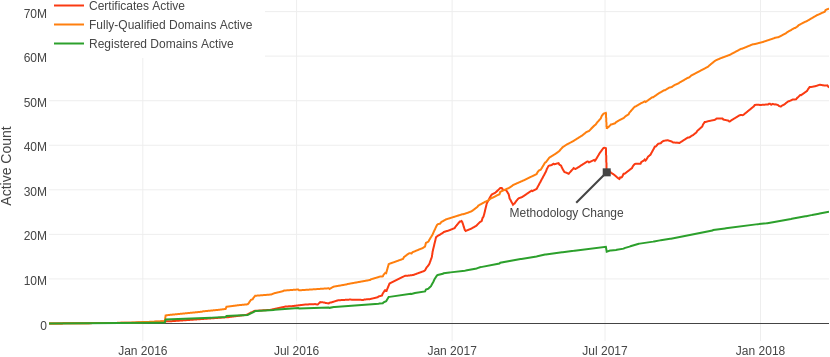
\includegraphics[width=.905\textwidth]{figures/letsencryptusers.png}
    \caption{Let's Encrypt user development until mid 2018~\cite{letsencryptstats}}
    \label{fig:letsencrypt}
\end{figure}

This project is already immensely successful, providing over 50 Million active certificates, as of March 2018 (see
\Cref{fig:letsencrypt})
However, this system is not intended for the general population, since the validation challenges are not for end-user but for web servers.
X.509 certificates, as issued by Let's Encrypt, can generally be used for email security with S/MIME\@.
There is also a proposed extension to the ACME protocol by \citet{melnikovAcmeSmime}, but not in any conceivable way
supported by Let's Encrypt.
Instead they explicitly state in their FAQ\footnote{https://letsencrypt.org/docs/faq/#does-let-s-encrypt-issue-certificates-for-anything-other-than-ssl-tls-for-websites},
that they do not issue certificates for anything other than websites.

\section*{Previous Work at TUM}
How email encryption certificates can be managed in an organization has been studied by the TUM Secure Email and User
Certification Project, with the works
of~\citet{hauner2016interoperability, jagdish2016certservice, straub2016directoryservice, maier2015multidevice}.
Maximilian Meier explored secure email communication with multiple devices, where he analyzed the requirements of
users and surveyed different implementations, that try to satisfy those requirements.
Straub and Jagdish worked on a combined system, which allows storage and management of digital certificates using a Java
backend with a web frontend.
In their work, they created a basic system, which can be used to store and manage certificates, but does not integrate
well with existing infrastructure in organizations.
In the most recent work, Valentin Hauner surveyed systems to publish certificates via different exchange protocols.
